\documentclass[fyp]{socreport}
\usepackage{hyperref}
\usepackage{graphicx} % to insert images
\usepackage{float}
%%% code block setups
\usepackage[newfloat]{minted}
\usepackage{xcolor} % to access the named colour LightGray
\definecolor{LightGray}{gray}{0.9}
\usepackage{caption}
\newenvironment{code}{\captionsetup{type=listing}}{}
\SetupFloatingEnvironment{listing}{name=Code}
%%% code block setups
\usepackage{fullpage}
\usepackage{multirow}
\usepackage{longtable}

\begin{document}
\pagenumbering{roman}
\title{Competition Platform for AI Tasks}
\author{Tan Yuanhong}
\projyear{2021/22}
\projnumber{H247080}
\advisor{Dr. Akshay Narayan, Prof. Leong Tze Yun}
\deliverables{
	\item Report: 1 Volume
	\item Source Code: 1 Git Repository}
\maketitle
\begin{abstract}
TO-DO

\begin{project-nature}
	Implementation, Experimentation, Simulation
\end{project-nature}
\begin{keywords}
    \item Artificial Intelligence
	\item Machine Learning
\end{keywords}
\begin{implement}
	Ubuntu 20.04, Python 3.8, Django 4.0
\end{implement}
\end{abstract}

% \begin{acknowledgement}
%   I would like to thank my friends, families and advisors.
%   Without them, I would not have be able to complete this project.
% \end{acknowledgement}

% \listoffigures 
% \listoftables
\tableofcontents 

\chapter{Introduction}
With the increasing popularity in both artificial intelligence (AI) research and industry application, more and more institutions are considering AI education as an integral part of their computer science or even general education curriculum. However, in spite the algorithmic nature of AI education, there is surprisingly few platforms and tools to host AI competitions/assignments and automatically grade the submissions. Unlike traditional algorithm and data structure courses that have many online judges available (to name a few, \href{https://codeforces.com/}{Codeforces}, \href{https://open.kattis.com/}{Kattis}, \href{https://onlinejudge.org/}{UVa Online Judge}), AI courses often rely on arbitrary grading scripts or in-house solutions to host their assignments/contests. There are well-known data science competition platforms like \href{https://www.kaggle.com/}{Kaggle} that are suitable for prediction/classification tasks, but the area of reinforcement learning (RL) tasks \footnote{To be precise, here tasks mean environments that are typically used for RL algorithms. The differentiating characteristic of such tasks is that they are interactive (in contrast to comparing the output against the ground truth like what Kaggle and other traditional OJs do).} remains surprisingly untouched. Therefore, this project tries to fill the gap of evaluating algorithms that solve interactive tasks. We aim to provide a complete solution from building RL \footnote{Technically the evaluation model we use is suitable for almost all AI/ML tasks (including classification and regression), but we will focus on RL first since we already have Kaggle for classification/regression tasks.} environments, writing test cases, to eventually hosting these tasks on a massively scalable platform.

\chapter{Project Objective}
\section{Problem Statement}
RL tasks are important problems to solve within artificial intelligence. Unlike other tasks such as prediction and classification, there are very few tools/platforms for creating and hosting RL task assignment/competitions. The goal of this project is to provide a complete solution for RL algorithm evaluation that is extensible, scalable, and well-documented. It consists of four tightly integrated components (collectively called aiVLE 2.0):

\begin{enumerate}
    \item aiVLE \footnote{aiVLE is name for the grading system currently used in CS4246, more details about the old aiVLE (aiVLE 1.0) are covered in Section~\ref{ch:literature-review-related-work-ai-competition-platforms}} Gym: An OpenAI Gym \cite{openai-gym} compatible RL environment framework with agent-environment separation and official support for multi-agent tasks.
    \item aiVLE Grader: An auto grading framework for aiVLE Gym tasks.
    \item aiVLE Worker: A security sandbox to execute arbitrary code submissions safely in a controlled environment, and a massively scalable worker client for evaluation.
    \item aiVLE Web: A web application for hosting RL competitions.
\end{enumerate}

\section{Motivation}
Courses like CS4246, which teach AI, and are different from traditional programming/algorithm courses, need a system to automate the process of collecting and evaluating programming assignments on AI tasks. aiVLE (AI Virtual Learning Environment) is the inspiration and foundation of this project – it is an RL task evaluation system built by the CS4246 teaching team since 2019. We will call the old aiVLE as aiVLE 1.0 henceforth\footnote{Do note that aiVLE 1.0 refers to the system as a whole –- it does not refer to any specific component (e.g., web, runner, runner-kit).}. aiVLE 1.0 provides instant feedback on programming assignments that require varied computational power such as GPU or other specialized processing units. However, aiVLE 1.0 has many pain points. For example, it lacks extensibility (e.g., does not support multi-agent task), scalability (e.g., no concurrency safety for many workers), and documentation for more courses to make use of the platform. As for another similar platform called Botzone~\cite{botzone}, although it’s built for external users, limitations like no GPU support and no common interface make it unviable for many tasks.
Secondly, an open source RL competition platform with good documentation and software engineering best practices has potential impact beyond education purposes. On the one hand, such a platform could also be useful for benchmarking AI algorithms – the consistency required for grading assignments is perfect for comparing research as well. On the other hand, examples like AlphaGo~\cite{alphago} proves the effectiveness of combining supervised learning from past match data with unsupervised RL – match history collected on the platform could be useful for training models for corresponding tasks. 
Lastly, there is demand for such a platform. Both CS3243 and CS4246 have assignments on RL algorithms. And even for many non-RL chapters such as brute force or informed search, satisfiability problems, the techniques could also be used to solve RL tasks. It is a safe bet that such a platform will benefit many AI courses (including CS2109S and CS3244) by using it alongside platforms like Kaggle to cover most AI algorithm evaluation scenarios.

\section{Roadmap}
There are three stages planned for this project:
\subsection{Stage 1: Framework}
Before developing the web platform for hosting the competitions, we first need frameworks for 1) creating environment and 2) evaluating agent’s performance – aiVLE Gym and Grader respectively. These frameworks are independent from the web platform, therefore could be used separately for other education or research purposes as well.
Besides platform-independent frameworks, a security sandbox, aiVLE Worker, is also necessary for hosting competitions. These three frameworks will be implemented in the mentioned order as the latter have dependency on the former.
\subsection{Stage 2: Platform}
With the frameworks ready, the second stage is to have a web platform that achieves basic online judge functionality, which includes but is not limited to: 1) user registration and authentication, 2) creating/joining courses, 3) creating/modifying/submitting to tasks, 4) showing the evaluation result. The target of this stage is to have a minimum viable product that CS4246 can use to host single-agent assignments with GPU-accelerated evaluation.
\subsection{Stage 3: Beyond CS4246}
Stage 1 and 2 provide a solid foundation for further extension and exploration, but primarily focus on delivering features that facilitate CS4246 teaching. Stage 3 aims to further extend the use case of our web platform, possibly to research and teaching of multi-agent systems, human-in-the-loop computing, and hosting ranked AI/RL competitions. Beyond education, we may also use the framework to build a test bed for RL algorithms and host the benchmark on the same platform for researchers.

\chapter{Literature Review}
\label{ch:literature-review}
\section{Background}
\subsection{Reinforcement Learning Tasks}
Reinforcement learning (RL) is a branch of machine learning that maps observations (possibly with history as well) to actions such that certain metrics are maximized~\cite{sutton-barto}. The metrics which agents try to maximize are called a reward or reinforcement, thus the name “reinforcement” learning. In a broader sense, any AI task is RL task: we can generalize any input as the observation, any output as the action and any target as the reward. But for the sake of simplicity, in this report, by RL task we mean sequential decision problems (SDP), where the outcome of agent’s decision depends on a sequence of decisions~\cite{russell}.

A sequential decision problem is fully described by state space, action space, transition model and a reward function~\cite{russell}. A transition model is a function that maps (current state, history states, action) to a probability of reaching any possible state. If the transition model does not depend on history state, we call it Markovian as the probability only depends on the current state instead of the history of all earlier states. A reward function maps current state \footnote{Reward function may also depend on action and next state, but one that only depends on the current state is the most common variant, and this difference is not fundamental.} to a numerical reward.

The solution to a sequential decision problem is called a policy. It is a function that maps current state (and sometimes history states) to an action. We always assume that the domain of policy function is the entire observation space so that the agent knows what action to take under any possible circumstance. The goal of RL algorithms is to come up with such policy functions that maximize their expected reward under different settings (e.g., unknown underlying transition model, partial observability, etc.).

From the definition of sequential decision problems, we can summarize the following execution loop of any typical SDP:

\begin{figure}[htp]
    \centering
    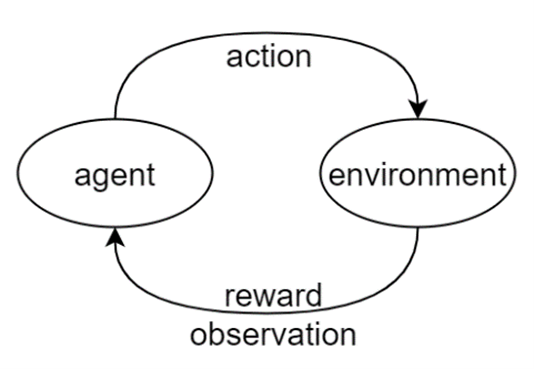
\includegraphics{images/obr-loop.png}
    \caption{Action-observation-reward loop}
    \label{fig:obr-loop}
\end{figure}

In other words, the environment implements the transition model $P\left(s_j\middle| s_i,a\right)$ and reward function $r\left(s_i\right)$ and returns the next observation $o_j$ and reward $r_j$ to the agent, after which the agent takes another step of action $a_{j+1}$ based on $\left[o_j,o_{j-1},\cdots,o_0\right]$ and $\left[r_j,r_{j-1},\cdots,r_0\right]$. Note that $o_i$ and $s_i$ may or may not be the same depending on whether the environment is fully observable.

\subsection{Reinforcement Learning Environment Frameworks And Collections}
RL research, like many computer science topics, requires concretizing the theory with implementation and experiments as they are equally important. That is where RL environment frameworks and collections like the Arcade Learning Environment (ALE)~\cite{ale} and OpenAI Gym~\cite{openai-gym} come into play. Such an effort is incredibly important for the rapid growth of the RL community: it not only saves researchers a lot of emulation development time, but also provides benchmark environments to evaluate RL tasks similar to how CIFAR-10~\cite{cifar-10} provides benchmark datasets in image classification. A typical OpenAI Gym agent code is structured as below:

\begin{code}
\begin{minted}[
frame=lines,
framesep=2mm,
baselinestretch=1.2,
bgcolor=LightGray,
fontsize=\footnotesize,
linenos
]{python}
import gym

env = gym.make('CartPole-v0')
for i_episode in range(100):
    observation = env.reset()
    for t in range(100):
        action = decide(observation, reward)
        observation, reward, done, info = env.step(action)
env.close()
\end{minted}
\captionof{listing}{OpenAI Gym agent example}
\label{code:gym-agent}
\end{code}

Besides collecting many classical environments as a benchmark package, an important contribution of OpenAI Gym is its widely accepted application programming interface (API). This common interface proves to be sufficient for not only hundreds of self-contained environments included in OpenAI Gym, but also thousands more third-party environments. When it comes to turning retro video games to RL environments, Gym dominates the game by eventually having ALE adopt its API and merge into Gym. Moreover, as if conquering Atari2600 is not enough, Gym Retro \cite{gym-retro} adds even more emulated systems such as Nintendo Game Boy and Sega Genesis to Gym. Therefore, it is safe to say that following this interface gives us enough flexibility to implement most of the desired environments.

From the source code of OpenAI Gym, a compatible environment needs to implement the methods and attributes shown in Figure~\ref{fig:gym-class}:

\begin{figure}[htp]
    \centering
    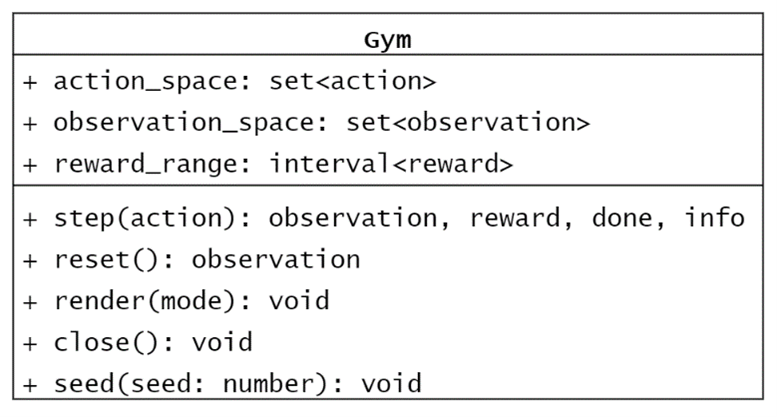
\includegraphics{images/gym-class.png}
    \caption{OpenAI Gym Class Diagram}
    \label{fig:gym-class}
\end{figure}

Authors of OpenAI Gym listed multi-agent as a future direction when they published the paper in 2016. However, as of 2021, there is still no official support for multi-agent tasks. There are some third-party environments that support multi-agent tasks, like ma-gym \cite{magym}. These implementations usually convert multi-agent observation, reward, and action into a vector, length of which is equal to the number of participating agents in the environment.

\section{Related Work}

\subsection{Online Judging System}
Online judges first emerged to address the problem of automatically grading programming assignments conveniently, fairly and securely \cite{RN4}. Without any manual intervention once the system is configured properly, online judge systems need to handle 1) receiving submissions, 2) compiling and executing source codes, 3) comparing outputs against the correct answers, 4) logging the result. For fairness, RAM and CPU usage will be monitored and limited. Usually, there is a hard time limit after which any submission will be forced to terminate. For security, execution of arbitrary submission needs to be contained in a safe environment with heavily restricted privilege levels such that only necessary operations are allowed, any other attempt (e.g., accessing the network, read/write on filesystem, etc.) will be blocked and preferably reported to the system administrator. 

Among all the challenges in building a successful online judge, security is probably the most technically difficult aspect. Some online judges were used in an exam setting where students had to use dedicated terminals for access, and a system administrator is involved in monitoring the security issues \cite{10.1145/384267.305835}. For automated security measures, there are generally two approaches: 1) source code or binary scanning, and 2) operating system level access control. 

Source code or binary scanning has no runtime performance penalty, but it requires an exhaustive check on all possible malicious tokens/system calls. It is unrealistic to have a perfectly secure source code scanner and every new supported language \footnote{A “new” language does not have to be a completely new one. If new keywords or new compiler version is introduced, there could possibly be new security implications.} requiring a new set of scanning rules makes this approach non-sustainable \cite{RN4}. Besides, it is impossible to scan the binary for programs written in a dynamic programming language such as Python as they execute inside an interpreter.

Access control based on operating system kernel security features is much more foolproof and widely applicable. Such techniques are also called OS-level virtualization because from the perspective of programs inside a ``namespace'', it can only see partial filesystem and devices that are assigned to this “namespace”. Since the introduction of user namespaces in Linux kernel 3.8, containerization technology has become increasingly popular to provide isolation between processes while being able to share nearly all hardware resources with minimal performance overhead \cite{RN16}. 

With the rapid growth of cloud and distributed computing, there are also novel online judges that attempt to adopt these cutting-edge technologies. A distributed online judge architecture tries to address the problem of scalability: an online judge needs to execute student submissions, and with more students and courses, computation required grows linearly. It is difficult to scale up (making computers more powerful) but easy to scale out (having more computers) especially in recent years with the emergence of cloud computing \cite{RN17}. Evaluating AI tasks has an even stronger demand for horizontal scalability as neural networks or sophisticated searching algorithms are notoriously computationally heavy. Notable implementations of distributed online judge include MetaOJ~\cite{metaoj}, which separates data storage, web application and judgers into three separate components that can be deployed to the cloud independently (Figure~\ref{fig:metaoj}).

\begin{figure}[H]
    \centering
    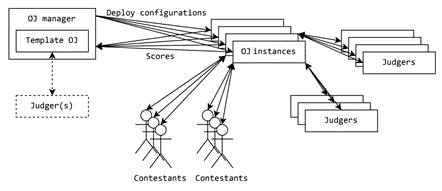
\includegraphics{images/metaoj.png}
    \caption{MetaOJ architecture}
    \label{fig:metaoj}
\end{figure}

\subsection{ML/RL Benchmark Platforms}
In contrast to competition platforms on the education side, researchers are more interested in a benchmark platform that provides a collection of tasks to compare different RL algorithms. Such benchmarks are crucial for reproducible and verifiable research in RL. According to~\cite{RN20}, an interpretable and reproducible experiment consists of four parts: algorithm, parameters, evaluation method and dataset. For a benchmark, evaluation method and dataset are fixed while contributors will compare different algorithms and parameters. In the context of RL benchmark, this means packaging the simulation environment and evaluation metrics behind a simple set of common interfaces for both training and testing.

However, as machine learning models (along with their training processes) get much more sophisticated, reproducibility is affected by not only those four points – random seeds, version of external libraries and even specific model of CPU/GPU could greatly affect the result of the same code \cite{RN21}. Therefore, according to “Ten Simple Rules for Reproducible Computational Research” by \cite{RN22}, for an RL benchmark platform to be reproducible, it should also: 1) have strict versioning \footnote{Meaning “any” change to the implementation of either environment or evaluation metrics should be reflected in a different version number. This also includes changes to the version of external dependencies.} of environments and evaluation metrics; 2) use deterministic methods whenever possible and fix random seeds throughout the process; 3) have a record of all raw data.
Considering the criteria listed above, OpenAI Gym (Brockman et al., 2016) is possibly one of the closest to an ideal benchmark: it explicitly embraces strict versioning, has an interface to fix random seeds, and includes many well-accepted tasks. Unfortunately, it only handles the simulation side of RL benchmark while leaving the evaluation to the users. For a successful ML benchmark platform like Kaggle, it not only provides dataset (environment in RL) but also enforces common evaluation criteria on all submissions so that algorithms are truly comparable.

\subsection{AI Competition Platforms}
\label{ch:literature-review-related-work-ai-competition-platforms}
In both sections Introduction and Project Objective, we mentioned that there are few RL task competition platforms. The available ones have pain points that make them unviable for many use cases. In this section, we compare aiVLE 1.0, an internally developed platform for CS4246 as a baseline of improvement for this project.
aiVLE 1.0 addresses the need for evaluating an OpenAI Gym agent in a GPU-accelerated environment. The architecture of aiVLE 1.0 is illustrated in Figure~\ref{fig:aivle-1-arch}:

\begin{figure}[H]
    \centering
    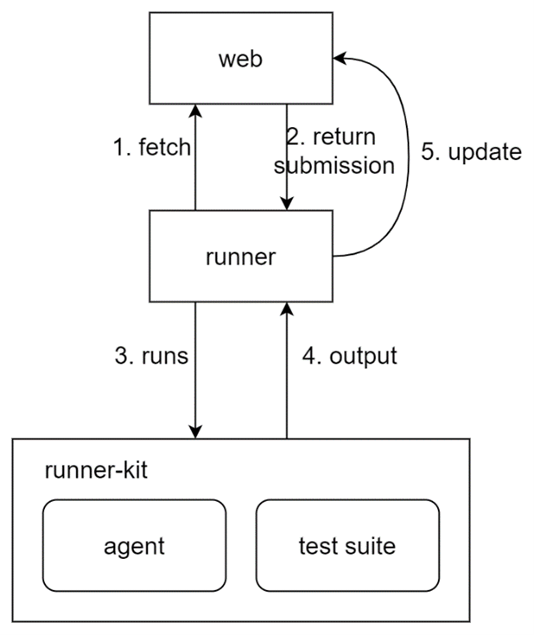
\includegraphics{images/aivle_1_arch.png}
    \caption{Architecture of aiVLE 1.0}
    \label{fig:aivle-1-arch}
\end{figure}

Due to urgency and time constraints, the author of aiVLE 1.0 prioritized “making it work” over “doing it right”, which leaves us four pain points\footnote{The list here is not exhaustive: more limitations and considerations will be discussed in Implementation Progress section, along with solutions to these pain points.} that impact its extensibility:

\begin{enumerate}
    \item Lack of documentation. For example, 1) deployment documentation for the runner instances (programs that evaluate student submissions), 2) architecture overview of each component and the entire system, and 3) inline documentation such as function usage, class definition. Without these documentation, new developers and users will take a much longer time to adopt and contribute to the system. 
    \item Need more coverage of software engineering best practices such as proper level of abstraction, and avoiding lengthy functions/files for interpretability, etc.
    \item No frontend-backend separation. Navigating and understanding the codebase is difficult as there is no clear boundary between frontend and backend code. Moreover, using JavaScript for interactivity would make the codebase look even more convoluted.
    \item No multi-agent support.
\end{enumerate}

For scalability, lack of proper task queue makes it difficult to scale aiVLE 1.0 to more machines: its workers get evaluation tasks by requesting server for the latest submissions \textit{periodically}. Worker-side polling has risks for traffic congestion and race condition, and the consequent lack of load balancing further hurts aiVLE 1.0’s potential to scale well with more workers – more details are covered in section 4.4.2.


\chapter{Design and Implementation}
\label{ch:design-and-impl}
Referring to the roadmap of this project, during the first semester I finished stage 1 (framework) and stage 2 (platform). Due to the page length restriction, I am providing an overview and one notable design detail of these subprojects in this report. Additional details on API documentation and design considerations can be found in these external documents:
\begin{enumerate}
    \item \href{https://yuanhong.larksuite.com/docs/docusSYdnLXZBojin39b8DGzKMT}{Gym} (Password: mLpj)
    \item \href{https://yuanhong.larksuite.com/docs/docuseeHRJWAMV3p3uL7yYCOeYx}{Grader} (Password: ZELI)
    \item \href{https://yuanhong.larksuite.com/docs/docussD8ik4yBXShA5kPyRGhgdg}{Worker} (Password: qgF2)
    \item \href{https://yuanhong.larksuite.com/docs/docusfWZk1oYG8qkEMG7y2oxkye}{Web} (Password: Z3Wn)
\end{enumerate}

Following the nomenclature defined in Section~\ref{ch:literature-review-related-work-ai-competition-platforms}, we will call the new system aiVLE 2.0 henceforth. Do note that aiVLE 2.0 also refers to the new system architecture as a whole – every subproject has an independent versioning that does not necessarily share the major revision number 2. This is because components like aiVLE Gym and aiVLE Grader does not exist in aiVLE 1.0.

\section{aiVLE Gym - Separating Agents from Environment}
\label{ch:aivle-gym}
I have released a stable version of aiVLE Gym with all planned features implemented. \href{https://github.com/edu-ai/aivle-gym}{The source} consists of ~1K lines of code, including several example environments and full documentation.

\subsection{Motivation}
aiVLE Gym makes multi-agent competition possible by separating agents from the environment. In a two-agent OpenAI Gym task, we write agent code as shown in Code~\ref{code:two-agent-example}:

\begin{code}
\begin{minted}[
frame=lines,
framesep=2mm,
baselinestretch=1.2,
bgcolor=LightGray,
fontsize=\footnotesize,
linenos
]{python}
env = gym.make("PongDuel-v0") # Two-player Ping Pong game
for ep_i in range(100):
    done_n = [False for _ in range(env.n_agents)]
    ep_reward = 0
    obs_n = env.reset()
    env.render()
    while not all(done_n):
        action_0 = decide_0(obs_n[0], reward_n[0])
        action_1 = decide_1(obs_n[1], reward_n[1])
        action_n = [action_0, action_1]
        obs_n, reward_n, done_n, info = env.step(action_n)
        ep_reward += sum(reward_n)
        env.render()
    print('Episode #{} Reward: {}'.format(ep_i, ep_reward))
env.close()
\end{minted}
\captionof{listing}{OpenAI Gym agent example}
\label{code:two-agent-example}
\end{code}

Note that in a multi-agent scenario, observation, reward and done are all vectors - each element corresponds to one of the agents. Similarly, when you call env.step(), you should provide actions for every agent in this simulation. Such design is acceptable when we perform these multi-agent experiments offline. However, in a competition setting, when it comes to multi-agent tasks, you cannot make decisions for your opponent agents. Therefore, separating agents from the environment simulation is necessary. From the perspective of each agent, it is just like a single-agent environment – the only difference is that the environment is affected by actions taken by other agents as well. Figure~\ref{fig:opanai-gym-multi-arch} and Figure~\ref{fig:aivle-gym-multi-arch} show the architectural differences between OpenAI Gym and aiVLE Gym (each colored box represents a separate process; solid arrows represent inter-process communication):
\begin{figure}[H]
    \centering
    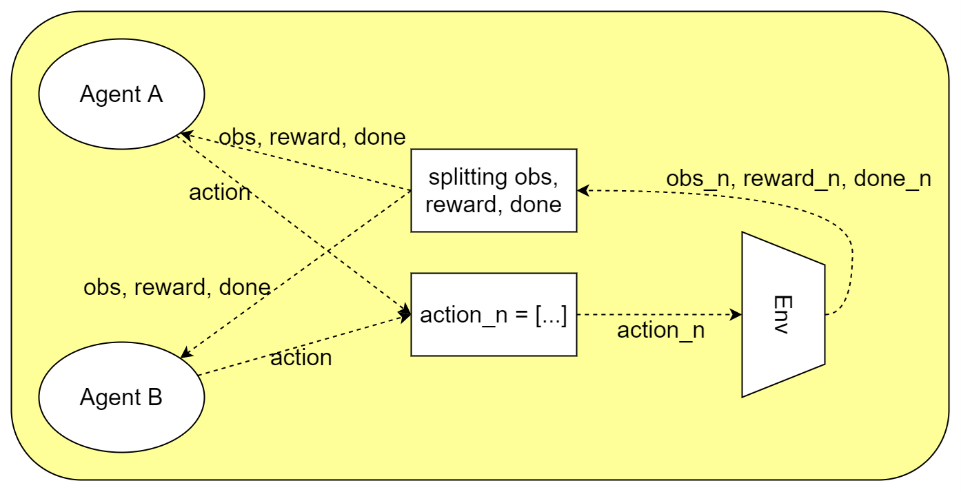
\includegraphics{images/opanai-gym-multi-arch.png}
    \caption{Multi-agent Architecture for OpenAI Gym}
    \label{fig:opanai-gym-multi-arch}
\end{figure}
\begin{figure}[H]
    \centering
    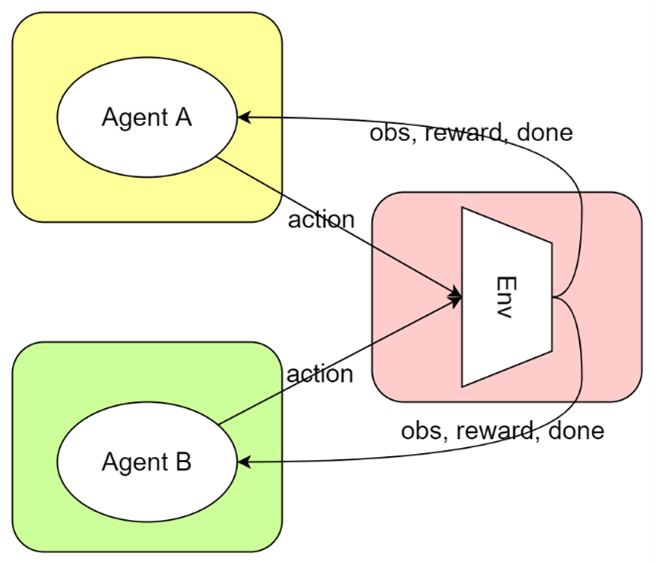
\includegraphics{images/aivle-gym-multi-arch.png}
    \caption{Multi-agent Architecture for aiVLE Gym}
    \label{fig:aivle-gym-multi-arch}
\end{figure}

\subsection{Design Goal}
Unless mentioned otherwise, all design goals in the following sections are achieved in the released implementation. 
The design goal of aiVLE Gym is to keep full compatibility with OpenAI Gym on the agent side. On the environment side, it lets you convert from existing OpenAI Gym environments with little adaptation. More specifically:
In single-agent case, on the agent side, traditional environment (simulation happens within agent process) and aiVLE environment (simulation happens outside of agent process) should be interchangeable. On the environment side, author can reuse existing OpenAI Gym compatible environment by implementing a serializer that serializes \texttt{action}, \texttt{observation}, and \texttt{info} to JSON compatible objects.
In multi-agent case, on the agent side, the APIs behaves just like normal single-agent OpenAI Gym environment (i.e., interchangeable). On the environment side, author can reuse existing ma-gym~\cite{magym} environment by implementing a serializer along with several metadata fields. 

\subsection{Agent-Environment Communication}
Since agents and environments are separated, there needs to be a communication channel between the two. aiVLE Gym uses a lightweight yet high-performance messaging library ZeroMQ~\cite{zeromq}, which has comprehensive support for many synchronous and asynchronous messaging patterns that are essential to this project. There are two primary challenges for multi-agent tasks when it comes to agent-environment communication:
\begin{enumerate}
    \item The judge should receive and respond to requests asynchronously - it needs to wait for all agents' actions before stepping forward in the environment, then decide what observations/rewards/done to respond to each of the agents.
    \item Certain operations (e.g., reset) must be performed strictly once for each episode, but since each agent will initialize the episode on their own, judge-side will unavoidably receive multiple requests.
\end{enumerate}

To summarize, the judge-side environment needs to implement a "barrier" synchronization mechanism that not only realizes synchronous rendezvous of agent requests, but also performs additional tasks upon the "first-comer" and "last-leaver". 

Therefore, we propose the deterministic finite automaton (DFA) as shown in Figure~\ref{fig:aivle-gym-multi-dfa}:
\begin{figure}[H]
    \centering
    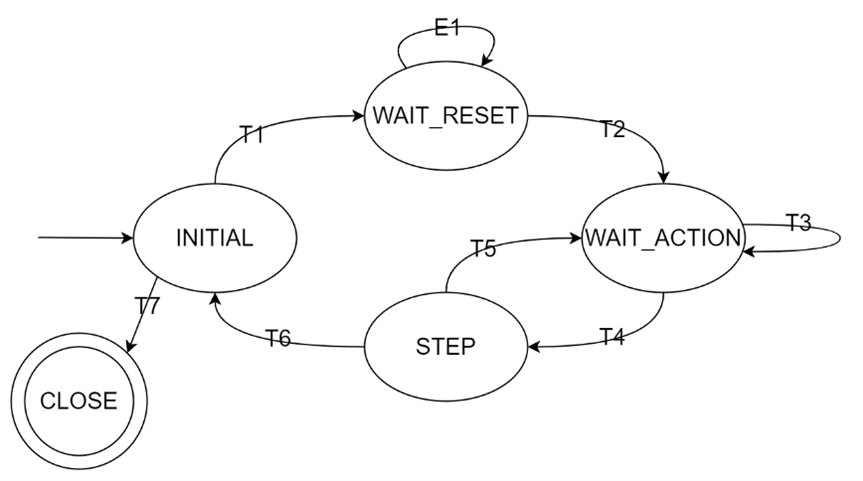
\includegraphics{images/aivle-gym-multi-dfa.png}
    \caption{aiVLE Gym Multi-agent Environment Communication Automaton}
    \label{fig:aivle-gym-multi-dfa}
\end{figure}

This DFA is key to keeping complicated communication details transparent to both agent and environment logic – both can write common synchronous code while the framework deals with the underlying asynchronous logic. Details of this DFA and messaging patterns involved can be found in the \href{https://google.com}{aiVLE Gym appendix}.

\section{aiVLE Grader - Evaluating Agents Using Test Suites}
\label{ch:aivle-grader}
I have released a stable version of aiVLE Grader with 1) normal OpenAI Gym, 2) aiVLE Gym single-agent, and 3) aiVLE Gym multi-agent environment support. The codebase consists of ~600 lines of framework code and ~300 lines of example test suites for all three supported frameworks.

\subsection{Design Goal}
Unlike competitive programming style problems or machine learning prediction tasks, evaluating RL agents is much more complicated than comparing students’ output against a standard answer. With the common programming interface provided by OpenAI/aiVLE Gym, on top of which, we may also create a framework that standardizes/modularizes the initialization, execution, and conclusion of RL agent evaluation. The ultimate goal of this framework, when writing a grader for agents in any OpenAI/aiVLE Gym environment, is to:
\begin{enumerate}
    \item Make the built-in components so complete that for most use cases using built-in ones would be sufficient.
    \item Make each component self-contained without complicated inter-dependencies (i.e., following the single responsibility principle) when writing a custom component.
\end{enumerate}

\subsection{Key Abstractions}
There are three key abstractions to aiVLE Grader: \textit{agent}, \textit{evaluator}, and \textit{test} case.
\textit{Agent} only has two methods: "reset" to reset internal states, "step" to return an action from provided observation. It is flexible enough to allow agents to memorize the history, whilst restrictive enough to prohibit agents from modifying the innerworkings of the environment.
\textit{Evaluator} records the entire execution process and produces a score when the session terminates. It utilizes the common pattern of most RL tasks (see Figure~\ref{fig:obr-loop}): each session consists of many episodes, and each episode consists of many concrete steps. By inserting hook functions to these critical points, an evaluator practically records everything about the evaluation session. 
\textit{Test case} is a bootstrap for evaluation sessions. It wraps \textit{agent}, \textit{environment}, and \textit{evaluator} along with necessary initialization parameters into an object with one simple “evaluate” method. It also offloads certain chore (e.g., runtime limit) away from the user.
\begin{figure}[H]
    \centering
    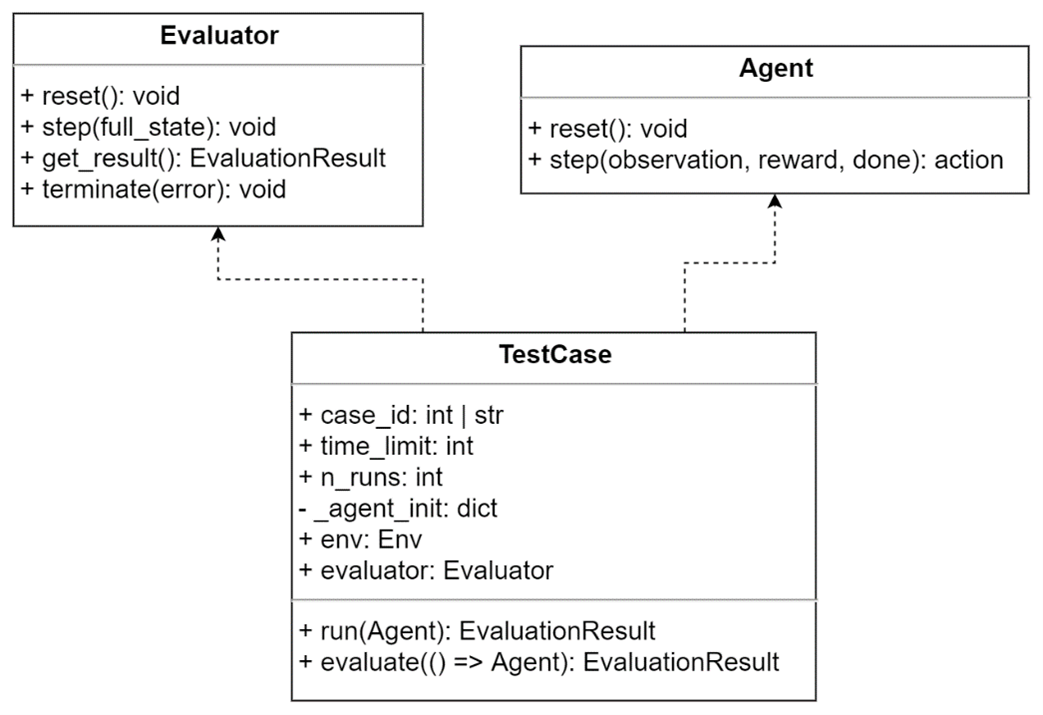
\includegraphics{images/aivle-grader-class.png}
    \caption{Class Diagram for aiVLE Grader}
    \label{fig:aivle-grader-class}
\end{figure}

\section{aiVLE Worker - Secure and Scalable Grading Client}
\label{ch:aivle-worker}
I have released a stable version of aiVLE Worker with an active CPU-only instance deployed on the server along with aiVLE Web. It is also tested on GPU machines for CUDA compatibility (GTX 1050Ti for CUDA 10, RTX 3070 for CUDA 11). The codebase consists of ~600 LoC, also with examples and full documentation.

\subsection{Design Goal}
As the section title suggests, security and scalability are what aiVLE worker aims to achieve. For security, the implementation is expected to achieve:
\begin{enumerate}
    \item File access restriction: agent program should have no access to directories that may contain sensitive data (e.g., private keys), and should have read only access to files necessary for its execution (e.g., Python binary, dependencies, agent, and environment source code).
    \item Network restriction: agent program should have no access to the Internet. Otherwise, (1) it may benefit from extra computation resources; (2) it may send out confidential runtime details (e.g., configuration of simulation environment) that allow users to fine-tune their program; both of which make the competition unfair.
    \item Resource limit, including RAM limit, CPU affinity (core count) and CPU time limit.
\end{enumerate}

As for scalability, it depends on both the scheduling on the server-side and the execution on the worker-side. In the context of scaling workers easily, a client that requires little permission and setup would be extremely helpful – so that we can deploy the worker on shared GPU servers or even lab machines. What we expect from this solution are:
\begin{enumerate}
    \item Managed concurrency  (work-in-progress): it should be able to run as many evaluation jobs concurrently as the hardware resource permits, while being able to detect and terminate processes that consume excessive RAM/VRAM.
    \item Minimal permission requirement: if we have access to run the submission locally, the environment should be able to operate as a worker node (i.e., sudo is not required).
    \item Minimal dependency requirement: any Linux machine with Python/Virtualenv/Pip should be able to run the worker client.
    \item Moderate overhead: compared to traditional OJ, aiVLE can trade some overhead (both startup and runtime) for absolute essentials like GPU support. However, to achieve a certain level of throughput, crazy warmup time like several minutes is still unacceptable.
\end{enumerate}

\subsection{Security Solution}
For security, I compared three mainstream security solutions: 1) virtual machine (VM) such as Virtualbox, 2) container such as Docker/Podman, and 3) sandbox such as Firejail. The main areas of interest are compared in Table~\ref{tab:security-solutions}:

\begin{table}[H]
\centering
\begin{tabular}{|c|c|cc|c|}
\hline
\multirow{2}{*}{} & \textbf{VM} & \multicolumn{2}{c|}{\textbf{Container}} & \textbf{Sandbox} \\ \cline{2-5} 
 & VirtualBox & \multicolumn{1}{c|}{Docker} & Podman & Firejail \\ \hline
\textbf{Rootless} & No & \multicolumn{1}{c|}{Yes} & Yes & Yes \\ \hline
\textbf{Level of isolation} & Very high & \multicolumn{2}{c|}{High} & Medium \\ \hline
\textbf{Overhead} & High & \multicolumn{2}{c|}{Low} & None \\ \hline
\textbf{Startup time} & $\sim$15s & \multicolumn{2}{c|}{$\sim$3s} & $\sim$0.05s \\ \hline
\textbf{GPU support} & No & \multicolumn{2}{c|}{Yes, with NVIDIA container runtime} & Yes \\ \hline
\end{tabular}
\caption{Comparison of Mainstream Security Solutions}
\label{tab:security-solutions}
\end{table}

There are several must-haves for the candidate solution:

\begin{enumerate}
    \item GPU-support. Many recent RL algorithms are practically impossible to run without a GPU. This eliminates VM without PCI passthrough.
    \item Server needs to be shared. This eliminates VM with PCI passthrough as it requires exclusive access. This also eliminates Podman and Docker, as it prevents the GPU from being shared by any other container with root access.
\end{enumerate}

Therefore, Firejail is the only option left. I built a custom security profile to expose only the necessary file system and devices to processes inside the sandbox. I also used Firejail to impose CPU affinity and RAM usage limit on each sandbox.

\section{aiVLE Web - AI competition platform}
\label{ch:aivle-web}
aiVLE Web consists of a Django backend that is ~2K LoC and a React frontend that is ~2K LoC. An active instance is deployed on the server and is accessible from \href{https://aivle.leotan.cn/}{https://aivle.leotan.cn/} (frontend) and \href{https://aivle-api.leotan.cn/}{https://aivle-api.leotan.cn/} (API and admin panel).

\subsection{Design Goal}
There are three primary considerations to the design of aiVLE web: extensibility, scalability, and usability. 
Extensibility means the architecture should be flexible enough for future upgrades including but not limited to multi-agent task competition and real-time match spectate. Scalability means the platform should be able to spread the evaluation workload, which is obviously the most computationally heavy task, over hundreds of worker machines. Usability means the platform should provide all the features the users (e.g., CS4246 teaching team) need for a successful semester of teaching.
For details of how I achieved the other goals, please refer to the appendix of aiVLE Web. In this report, I will talk about the task queue mechanism that makes aiVLE 2.0 a massively scalable online judge.

\subsection{Highly Available and Fault Tolerant Task Queue}
\label{ch:aivle-web_highly-available-task-queue}
This is a continuation of scalability of (grading) workers. In the section for aiVLE worker, we addressed the problem of running the worker on as many computers as possible with as little configuration/permission as possible. Here we address the problem of 1) coordinating the communication between the workers and the backend server, and 2) distributing grading tasks to the workers efficiently for shorter waiting time and higher resource utilization.
\subsubsection{The Problem}
In original aiVLE, there was no concept of "task queue". All pending tasks are stored in the DB with the status "QUEUED". Communication between the worker (or runner as per the term used by original author) and server is \textit{half-duplex by polling}. In other words, the worker makes \textbf{periodic} requests to the server for new ungraded submissions:
\begin{figure}[H]
    \centering
    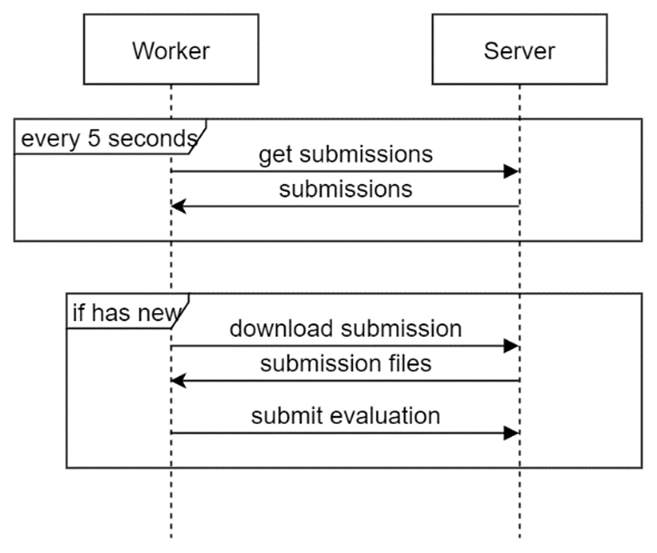
\includegraphics{images/aivle-web-old-task-queue.png}
    \caption{Old aiVLE “Task Queue”}
    \label{fig:aivle-web-old-task-queue}
\end{figure}
There are three critical limitations to this approach:
\begin{enumerate}
    \item Worker-side polling doesn't scale well: there is zero mechanism in orchestrating the timing and order of workers polling the server for new jobs. The severity of possible traffic spike (i.e., many workers poll the server at the same time due to lack of coordination) increases linearly with the number of worker nodes.
    \item Possible race condition: if two worker pull submissions at the same time, both will get the same ungraded submission. Such redundant work will get more significant with more worker nodes, which hurts the overall efficiency of the worker cluster.
    \item No concurrency on each worker: each individual worker only polls for new job when it has no submission to grade. In other words, each worker can only grade one submission at a time.
    \item No load balancing: the backend has no control over which worker grades which submission, therefore load balancing is virtually impossible
\end{enumerate}

\subsubsection{The Solution}
Similar to the idea of extracting the responsibility of data storage/management into a separate database backend, we delegate the messaging tasks to a message queue. Conceptually, message queue enables asynchronous communication between clients (who submit tasks) and workers (who finish tasks). Below is a diagram illustrating how the MQ-based task queue works:
\begin{figure}[H]
    \centering
    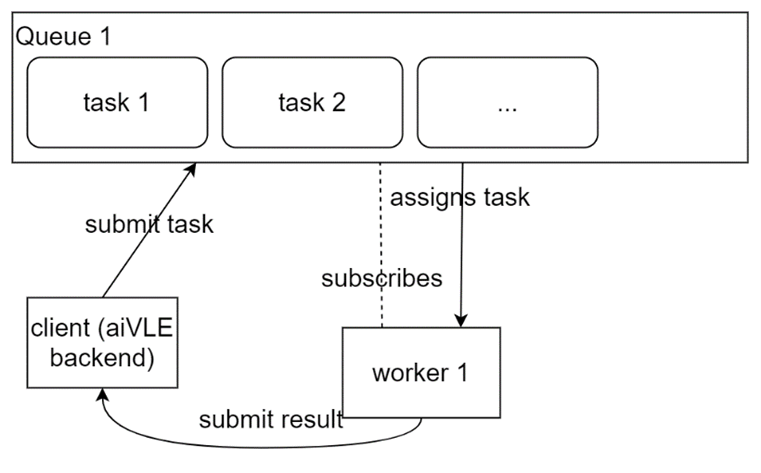
\includegraphics{images/aivle-web-mq.png}
    \caption{Message Queue Based Task Queue}
    \label{fig:aivle-web-mq}
\end{figure}
Every worker listens to one or more "queues", where the message broker is responsible for allocating tasks fairly among workers in each queue. When an evaluation job comes, aiVLE backend will submit the job to an appropriate queue (i.e., private queue if user has dedicated workers available, otherwise public CPU/GPU queue according to task specification) and wait for the assigned worker to submit evaluation result. The task will remain in the queue until it is processed (i.e., message queue is persistent). A randomly generated task ID is used to authenticate worker's submission – only the worker whom the broker assigned the task will have this ID. This approach not only reduces the number of requests to be O(n) where n is the number of evaluation jobs, but also ensures fair assignment of tasks among workers. Moreover, we also benefit from other standard features of MQ such as automatic retry and heartbeat checks.

\chapter{Deployment and Testing}
\label{ch:deployment-and-testing}
As mentioned in Section~\ref{ch:design-and-impl}, aiVLE 2.0, especially aiVLE Worker and aiVLE Grader, is designed to be highly scalable and easy to deploy. However, just like any distributed systems, being able to run the individual components on a single machine is one thing, having all the components cooperate on separate machines to achieve actual distribution is another story. Thus, to pave way for future production deployment, and to demonstrate the actual performance of such a distributed system, we performed a complete deployment using several SoC cluster nodes \footnote{Special thanks to the SoC compute cluster admins and Dr. Narayan for their help in securing these very powerful GPU nodes as shown later in Section~\ref{ss:deployment-environment}.} and did several experiments/benchmarks on the system.

There will be three sections to this chapter: 

\begin{itemize}
    \item Section~\ref{s:deployment} describes the deployment environment, deployment steps and issues we encountered before making the system fully functional on SoC.
    \item Section~\ref{s:load-balance-exp} describes the methodology and findings of load balancing among all worker nodes.
    \item Section~\ref{s:concurrency-exp} describes the methodology and findings of running multiple evaluation jobs concurrently on a \emph{single} worker node.
\end{itemize}

\section{Deployment}
\label{s:deployment}
Note that this deployment happened during the winter break (Nov 2021 to Jan 2022). Therefore some later updates to the aiVLE Web and Worker are not included during this deployment (most notably, the resource-sensitive load balancing related features). In specific, the exact versions used are (Git commit hash with GitHub link):
\begin{itemize}
    \item aiVLE Web: \href{https://github.com/edu-ai/aivle-web/commit/b346a68e30aa05656ae2e6cc106414bcba5430fd}{b346a68e30aa05656ae2e6cc106414bcba5430fd}
    \item aiVLE Worker: \href{https://github.com/edu-ai/aivle-worker/commit/647d767a72acf6c5f5ded533d77141ca91f4ef9d}{647d767a72acf6c5f5ded533d77141ca91f4ef9d}
\end{itemize}

\subsection{Environment}
\label{ss:deployment-environment}
aiVLE Worker is deployed on SoC compute cluster \texttt{xgpg0, xgpg1, xgpg2} with the following configuration:
\begin{itemize}
    \item Operating System (Code~\ref{code:deployment-os}): Ubuntu 20.04 LTS with Linux kernel version 5.4.0
    \item GPU (Code~\ref{code:deployment-gpu}): NVIDIA A100-PCI, Driver 495.29, CUDA 11.5
    \item CPU: 2x AMD Epyc 7352, in total 48 cores/96 threads, base clock 2.3GHz
    \item RAM: 256GiB DDR4
\end{itemize}

\begin{code}
\begin{minted}[frame=lines,framesep=2mm,baselinestretch=1.2,bgcolor=LightGray,fontsize=\footnotesize,linenos]{shell}
> cat /proc/version
Linux version 5.4.0-91-generic (buildd@lcy01-amd64-017) 
(gcc version 9.3.0 (Ubuntu 9.3.0-17ubuntu1~20.04)) #102-Ubuntu SMP Fri Nov 5 16:31:28 UTC 2021
\end{minted}
\captionof{listing}{Deployment Environment - Operating System}
\label{code:deployment-os}
\end{code}

\begin{code}
\begin{minted}[frame=lines,framesep=2mm,baselinestretch=1.2,bgcolor=LightGray,fontsize=\footnotesize,linenos]{shell}
> nvidia-smi 
Sat Jan  1 13:32:49 2022       
+-----------------------------------------------------------------------------+
| NVIDIA-SMI 495.29.05    Driver Version: 495.29.05    CUDA Version: 11.5     |
|-------------------------------+----------------------+----------------------+
| GPU  Name        Persistence-M| Bus-Id        Disp.A | Volatile Uncorr. ECC |
| Fan  Temp  Perf  Pwr:Usage/Cap|         Memory-Usage | GPU-Util  Compute M. |
|                               |                      |               MIG M. |
|===============================+======================+======================|
|   0  NVIDIA A100-PCI...  On   | 00000000:01:00.0 Off |                    0 |
| N/A   49C    P0    36W / 250W |      0MiB / 40536MiB |      0%      Default |
|                               |                      |             Disabled |
+-------------------------------+----------------------+----------------------+
\end{minted}
\captionof{listing}{Deployment Environment - GPU}
\label{code:deployment-gpu}
\end{code}

aiVLE Web is deployed on a \href{https://linode.com/}{Linode} Nanode 1GB VPS (virtual private server) with 1 virtual CPU core and 1 GiB of RAM.

\subsection{Steps}

To simulate the production deployment process, we scrapped the existing setups and started everything afresh. The following steps are sufficient for any deployment from the ground up:

\begin{enumerate}
    \item Prepare the message queue broker: either by installing \href{https://www.rabbitmq.com/}{RabbitMQ} or using cloud message queue provider such as \href{https://www.cloudamqp.com/}{CloudAMQP}. In our case, we installed RabbitMQ on the same VPS with aiVLE Web.
    \item Install and start aiVLE Web on the VPS.  \href{https://github.com/edu-ai/aivle-web#readme}{aiVLE Web Readme} describes this process in detail.
    \item Setup the users, courses, tasks in aiVLE Web via its RESTful API or Django admin panel.
    \item Prepare the worker nodes with necessary dependencies (i.e., Firejail, Pip, Virtualenv, CUDA drivers). In our case, we requested the cluster admins to install Firejail as all other dependencies are already available.
    \item Install and start aiVLE Worker on the worker nodes. \href{https://github.com/edu-ai/aivle-worker#readme}{aiVLE Worker Readme} describes this process in detail.
\end{enumerate}

\subsection{Issues and Solutions}
There are some issues we found during the deployment process. None of which is critical in a sense that we eventually found workarounds without modifying any existing codebase or design. But we think it is nonetheless useful to point them out here as potential users of this system is likely to encounter some of them as well.
\subsubsection{Switching broker from RabbitMQ to AWS SQS}
If the worker node resides behind a firewall that restricts access to certain ports (especially under a whitelist policy where only selected ports are available), then you are likely to find RabbitMQ unusable - its underlying protocol, Advanced Message Queuing Protocol (AMQP), uses port 5671/5672 by default. There are two possible solutions:
\begin{enumerate}
    \item Change RabbitMQ port to one that is allowed by the worker node firewall. Do note that AMQP is not based on HTTP/HTTPS, so when change the port to 80/443 you need to ensure that not only the broker server has those ports available, but also the worker node firewall DOES allow non-HTTP traffic via port 80/443.
    \item Switch RabbitMQ to HTTP/HTTPS-based broker such as \href{https://aws.amazon.com/sqs/}{AWS SQS}. Do note that this solution greatly affects the capability of Celery task scheduling - for example, remote worker control is impossible with SQS. As a result, later advanced features like resource-sensitive load balancing would not work under SQS.
\end{enumerate}
In our case, the SoC firewall blocks most ports on external IP address, and forcing RabbitMQ to use port 80 was futile. In the end we switched to AWS SQS as a workaround\footnote{It did not affect any existing functionality then - features such as resource-sensitive load balancing came later in the second semester.}.

\subsubsection{Firejail Version Requirement}
Firejail security profile is not forward compatible, and the latest Firejail version is determined by the OS version, therefore the default security profile of aiVLE Worker doesn't work on  \texttt{xgpd0} which has Ubuntu 16.04 installed. It works as expected on both Ubuntu 18.04 and Ubuntu 20.04 with their latest Firejail version respectively.
To avoid future confusions, we listed Ubuntu 20.04 as a requirement for aiVLE Worker on its Readme file.

\subsubsection{PyTorch Installation Issue with Latest nVIDIA GPU}
Although it has been two years since the launch of RTX 30-series GPU\footnote{The same applies to data center GPUs launched after RTX 30-series, such as nVIDIA A100 used in our deployment.}, PyTorch official PIP channel still hasn't supported CUDA 11 (which is the minimum CUDA version for 30-series GPU). So instead of 
\begin{code}
\begin{minted}[frame=lines,framesep=2mm,baselinestretch=1.2,bgcolor=LightGray,fontsize=\footnotesize]{shell}
pip3 install torch torchvision torchaudio
\end{minted}
\end{code}
we need to use
\begin{code}
\begin{minted}[frame=lines,framesep=2mm,baselinestretch=1.2,bgcolor=LightGray,fontsize=\footnotesize]{shell}
pip3 install torch==1.10.1+cu113 torchvision==0.11.2+cu113 \
torchaudio==0.10.1+cu113 -f \
https://download.pytorch.org/whl/cu113/torch_stable.html
\end{minted}
\end{code}

This means the author of the task needs to be aware of the CUDA version of their allocated grading machines, and adjust their \texttt{requirements.txt} accordingly.

\section{Load Balance Experiment}
\label{s:load-balance-exp}
Raw logs and analyzing scripts can be found in \href{https://github.com/edu-ai/aivle-experiment-logs}{aiVLE Experiment Logs Repo}. For correspondence between experiment setup and log file index, please refer to Table~\ref{tab:load-balance-exp}

\begin{table}[H]
\centering
\begin{tabular}{|c|c|c|c|c|c|}
\hline
\multicolumn{1}{|l|}{\begin{tabular}[c]{@{}l@{}}Web\\ log index\end{tabular}} & \multicolumn{1}{l|}{\begin{tabular}[c]{@{}l@{}}Worker\\ log index\end{tabular}} & \multicolumn{1}{l|}{Node count} & \multicolumn{1}{l|}{\begin{tabular}[c]{@{}l@{}}Concurrency \\ of worker\end{tabular}} & \multicolumn{1}{l|}{Submission count} & \multicolumn{1}{l|}{\begin{tabular}[c]{@{}l@{}}Concurrency \\ of submission\end{tabular}} \\ \hline
5 & 2 & 3 & 8 & 100 & 100 \\ \hline
6 & 3 & 2 & 8 & 100 & 100 \\ \hline
7 & 4 & 1 & 8 & 100 & 100 \\ \hline
\end{tabular}
\caption{Load Balancing Experiment Setup}
\label{tab:load-balance-exp}
\end{table}

\subsection{Methodology}
\label{ss:lb-exp-meth}
Since the evaluation task and all worker nodes are exactly the same, we have four parameters/variables to adjust:
\begin{enumerate}
    \item Node count: number of active nodes during the experiment.
    \item Concurrency of worker: maximum number of concurrent evaluation jobs allowed on \emph{each} worker node.
    \item Submission count: number of \emph{total} evaluation jobs submitted to the task queue.
    \item Concurrency of submission: maximum number of threads submitting jobs at the same time.
\end{enumerate}

In this section and Section~\ref{s:concurrency-exp}, submission count and concurrency of submission are both 100. This means before the first job is assigned to any of the worker nodes, 100 jobs are already queued. This is to ensure there will always be sufficient tasks for the workers to work on - if concurrency of submission is significantly smaller than the number of submissions, then the rate of submitting job may dictate the rate of workers finishing jobs, which is undesirable for our stress-oriented experiments.

For load balance experiment, we \textbf{fix concurrency on all workers to be 8}, measure \textbf{time taken} to finish 100 submissions with
\begin{enumerate}
    \item 1 node (\texttt{xgpg0})
    \item 2 nodes (\texttt{xgpg0,1})
    \item 3 nodes (\texttt{xgpg0,1,2})
\end{enumerate}

On the master server (aiVLE Web), we logged the critical phases of each submission with a timestamp, in specific, there is a timestamped record when
\begin{enumerate}
    \item received submission
    \item submitted to task queue
    \item task picked up by a worker
    \item task being worked on by a worker
    \item task terminated (finished or failed)
\end{enumerate}

The start time is defined to be the earlier of 1) the latest "received submission" record and 2) the earliest "task picked up by a worker" record. The finish time is defined to be the latest "task terminated" record. The total time is defined to be the difference between the finish time and the start time. The detailed method of calculating time taken to finish all submissions can be found in the \href{https://github.com/edu-ai/aivle-experiment-logs/blob/main/web/analyze.ipynb}{analyze script}.

On each worker node, we also logged the timestamped GPU utilization rate and VRAM usage periodically. This helps us understand whether all worker nodes are busy most of the time - unnecessary idling is a sign of poor load balancing.

\subsection{Results}

For the performance of load balancing, here are the times for each test case:
\begin{itemize}
    \item 1 nodes: 235.426s (baseline)
    \item 2 nodes: 128.261s (91.78\%)
    \item 3 nodes: 92.475s (84.86\%)
\end{itemize}

For the faireness of load balancing, here are the number of jobs assigned to each worker node (when there are more than one node):
\begin{itemize}
    \item 2 nodes: \texttt{\{'celery@xgpg0': 50, 'celery@xgpg1': 50\}}
    \item 3 nodes: \texttt{\{'celery@xgpg0': 34, 'celery@xgpg1': 36, 'celery@xgpg2': 30\}}
\end{itemize}

TODO

\section{Concurrency Experiment}
\label{s:concurrency-exp}
Raw logs and analyzing scripts can be found in \href{https://github.com/edu-ai/aivle-experiment-logs}{aiVLE Experiment Logs Repo}.For correspondence between experiment setup and log file index, please refer to Table~\ref{tab:concurrency-exp}

\begin{table}[H]
\centering
\begin{tabular}{|c|c|c|c|c|c|}
\hline
\multicolumn{1}{|l|}{\begin{tabular}[c]{@{}l@{}}Web\\ log index\end{tabular}} & \multicolumn{1}{l|}{\begin{tabular}[c]{@{}l@{}}Worker\\ log index\end{tabular}} & \multicolumn{1}{l|}{Node count} & \multicolumn{1}{l|}{\begin{tabular}[c]{@{}l@{}}Concurrency \\ of worker\end{tabular}} & \multicolumn{1}{l|}{Submission count} & \multicolumn{1}{l|}{\begin{tabular}[c]{@{}l@{}}Concurrency \\ of submission\end{tabular}} \\ \hline
7 & 4 & 1 & 8 & 100 & 100 \\ \hline
8 & 5 & 1 & 4 & 100 & 100 \\ \hline
9 & 6 & 1 & 2 & 100 & 100 \\ \hline
10 & 7 & 1 & 1 & 100 & 100 \\ \hline
\end{tabular}
\caption{Per-worker Concurrency Experiment Setup}
\label{tab:concurrency-exp}
\end{table}

\subsection{Methodology}
For explanation of parameters/variables, and the method of measuring total time please refer to Section~\ref{ss:lb-exp-meth}. For the per-worker concurrency experiment, we activate \textbf{only one} worker node, and measure \textbf{time taken} to finish 100 submissions with
\begin{enumerate}
    \item concurrency of worker = 1
    \item concurrency of worker = 2
    \item concurrency of worker = 4
    \item concurrency of worker = 8
\end{enumerate}

\subsection{Results}

\begin{itemize}
    \item concurrency = 1: 1558.811s (baseline)
    \item concurrency = 2: 859.237s (90.71\%)
    \item concurrency = 4: 422.744s (92.18\%)
    \item concurrency = 8: 235.426s (82.77\%)
\end{itemize}

\chapter{Future Plans}
\label{ch:future-plans}
\section{Support and Improvement}
As mentioned in Chapter~\ref{ch:design-and-impl}, I reached the targets set for the first two stages and has delivered a system that satisfies the basic requirements of CS4246 teaching. Despite our best effort, one semester is not enough to implement every feature that we can think of. Therefore, the first planned item for semester 2 is to support the use cases of aiVLE 2.0 and add more features.
For the framework (aiVLE Gym and Grader), there is an ongoing collaboration with Ho Hol Yin for a unified testbed for AI teaching and research (project ID: H247060). This will hopefully be the first concrete demonstration of these frameworks and I will support Hol Yin throughout his development and make improvements to my frameworks accordingly.
For the platform (aiVLE Worker and Web), CS4246 for the next semester will possibly transition to the new system. There will be more stress testing and security penetration testing for production use of the system. Bug fixes and quality of life improvements will be introduced on the fly when the system is in active use. There are also several new features planned for the next semester:

\begin{enumerate}
    \item More comprehensive evaluation queue support: currently any evaluation job is assigned to either public CPU queue or public GPU queue. We need to support private queue that is operated by external users when the platform goes public.
    \item Resource sensitive concurrency management: currently the number of concurrent jobs allowed on each worker is fixed. Although having worker-level concurrency itself is already a huge improvement over the old system, the goal is to dynamically adjust the concurrency limit to fully utilize the hardware without manual configuration.
    \item Platform support for two-agent tasks (e.g., Gobang, Go, Reversi, etc.): a matchmaker and Elo-based ranking system.
    \item Record and export match history.
    \item Visualization of match history.
    \item Course management interface. Current aiVLE 2.0 relies on default admin panels provided by Django and Django REST Framework, which are not particularly user-friendly.
\end{enumerate}

\subsection{Beyond AI Education}
Although the project is titled as a competition platform for AI education, half of its effort focuses on providing an easy-to-use and standardized RL environment framework and evaluation tool that natively supports multi-agent tasks. As suggested by my supervisors Prof. Leong and Dr. Narayan, there are several areas I might explore with these tools:
\begin{enumerate}
    \item Package the aiVLE Gym and dependencies to ensure software-level reproducibility – given a specific version of aiVLE environment, a Docker image will harden all dependency and driver versions.
    \item Extend aiVLE Gym to support inter-agent communication to fill the gap of benchmarking collaborative RL algorithms.
    \item Collect some classic multi-agent tasks and implement some classic RL algorithms on these tasks to validate the potential of using these frameworks as a benchmark for future tasks and algorithms. The collaboration with Hol Yin is relevant as well.
    \item Make aiVLE a one-stop solution of sharing RL environment and benchmarking RL algorithms by adding a section in the web platform for users to 1) submit environments, 2) submit and evaluate agents to respective environments, and 3) compare agent performance.
\end{enumerate}


\bibliographystyle{socreport}
\bibliography{socreport}

\appendix
\chapter{Code}

% \chapter{Proofs}
% In this appendix, we present alternate, longer, but more interesting proof 
% of correctness of our algorithm.  This proof is based on induction and proof
% by contradiction.
\end{document}
